% =============================================================================
%  FIVUCSAS — Poster variant: MODERN MINIMALIST
%  A0 portrait. Sans-serif, generous whitespace, single teal accent.
%  Compile:  pdflatex poster.tex && pdflatex poster.tex
% =============================================================================
\documentclass[a0paper,portrait]{tikzposter}
\tikzposterlatexaffectionproofoff
\geometry{paperwidth=841mm,paperheight=1189mm}

\usepackage[utf8]{inputenc}
\usepackage[T1]{fontenc}
\usepackage{lmodern}
\renewcommand{\familydefault}{\sfdefault}
\usepackage{microtype}
\usepackage{xcolor}
\usepackage{graphicx}
\graphicspath{{../../assets/}{./assets/}{./poster/assets/}}
\usepackage{fontawesome5}
\usepackage{qrcode}
\usepackage{tikz}
\usepackage{enumitem}
\usetikzlibrary{positioning,calc,arrows.meta,backgrounds}

% Official institutional crests (assets/)
\newcommand{\unicrest}[1][2.6cm]{
\includegraphics[height=#1,keepaspectratio]{marmara-university.png}}
\newcommand{\faccrest}[1][2.6cm]{
\includegraphics[height=#1,keepaspectratio]{muhendislik-fakultesi.jpg}}

% ---------- Minimalist palette (one accent, mostly grayscale) ----------------
\definecolor{MAccent}{HTML}{1E96A8}     % MarmaraTeal — single accent
\definecolor{MInk}{HTML}{1B1F23}
\definecolor{MGray}{HTML}{8E959B}
\definecolor{MGrayLite}{HTML}{ECEDEF}
\definecolor{MBg}{HTML}{FFFFFF}
\definecolor{MRule}{HTML}{C8CCD0}

% ---------- Theme: empty background, no block decoration ---------------------
\definelayouttheme{Minimalist}{
  \usecolorstyle[colorPalette=MinPal]{Default}
  \usebackgroundstyle{Empty}
  \usetitlestyle{Empty}
  \useblockstyle{Empty}
  \useinnerblockstyle{Default}
  \usenotestyle{Default}
}
\definecolorpalette{MinPal}{
  \definecolor{colorOne}{named}{MInk}
  \definecolor{colorTwo}{named}{MInk}
  \definecolor{colorThree}{named}{MAccent}
}
\usetheme{Minimalist}
\colorlet{backgroundcolor}{MBg}
\colorlet{framecolor}{MBg}
\colorlet{titlefgcolor}{MInk}
\colorlet{titlebgcolor}{MBg}
\colorlet{blocktitlebgcolor}{MBg}
\colorlet{blocktitlefgcolor}{MInk}
\colorlet{blockbodybgcolor}{MBg}
\colorlet{blockbodyfgcolor}{MInk}
\colorlet{innerblocktitlebgcolor}{MBg}
\colorlet{innerblocktitlefgcolor}{MAccent}
\usebackgroundstyle{Empty}

% ---------- Title (custom, very airy, logos flanking) ------------------------
\title{\parbox{0.96\linewidth}{\centering
  \begin{minipage}[c]{0.11\linewidth}\centering\unicrest[2.2cm]\end{minipage}\hfill
  \begin{minipage}[c]{0.76\linewidth}\centering
  {\fontsize{72}{72}\selectfont\bfseries\color{MInk}FIVUCSAS}\\[0.3em]
  {\Large\color{MGray}Face and Identity Verification Using Cloud-based SaaS}\\[0.2em]
  {\normalsize\color{MAccent}\textbf{---}}\\[0.2em]
  {\large\color{MInk}\textsl{Multi-tenant biometric authentication with active-liveness anti-spoofing}}
  \end{minipage}\hfill
  \begin{minipage}[c]{0.11\linewidth}\centering\faccrest[2.4cm]\end{minipage}
}}
\author{}
\institute{}

\begin{document}
\maketitle[width=\paperwidth, titletotopverticalspace=20mm]

% ---------- Author strip -----------------------------------------------------
\block[bodyoffsety=-25mm, bodyinnersep=2mm]{}{\centering
  {\large\color{MInk}Ahmet Abdullah Gültekin \quad\textcolor{MGray}{·}\quad Ayşe Gülsüm Eren \quad\textcolor{MGray}{·}\quad Ayşenur Arıcı}\\[0.3em]
  {\small\color{MGray}Advisor: Assoc.\ Prof.\ Dr.\ Mustafa Ağaoğlu \quad·\quad CSE4197 / CSE4198 \quad·\quad Spring 2025–2026}\\[0.3em]
  {\small\color{MGray}Marmara University · Faculty of Engineering · Department of Computer Engineering}
}

% ---------- KPI strip --------------------------------------------------------
\block[bodyoffsety=-5mm, bodyinnersep=8mm]{}{\centering
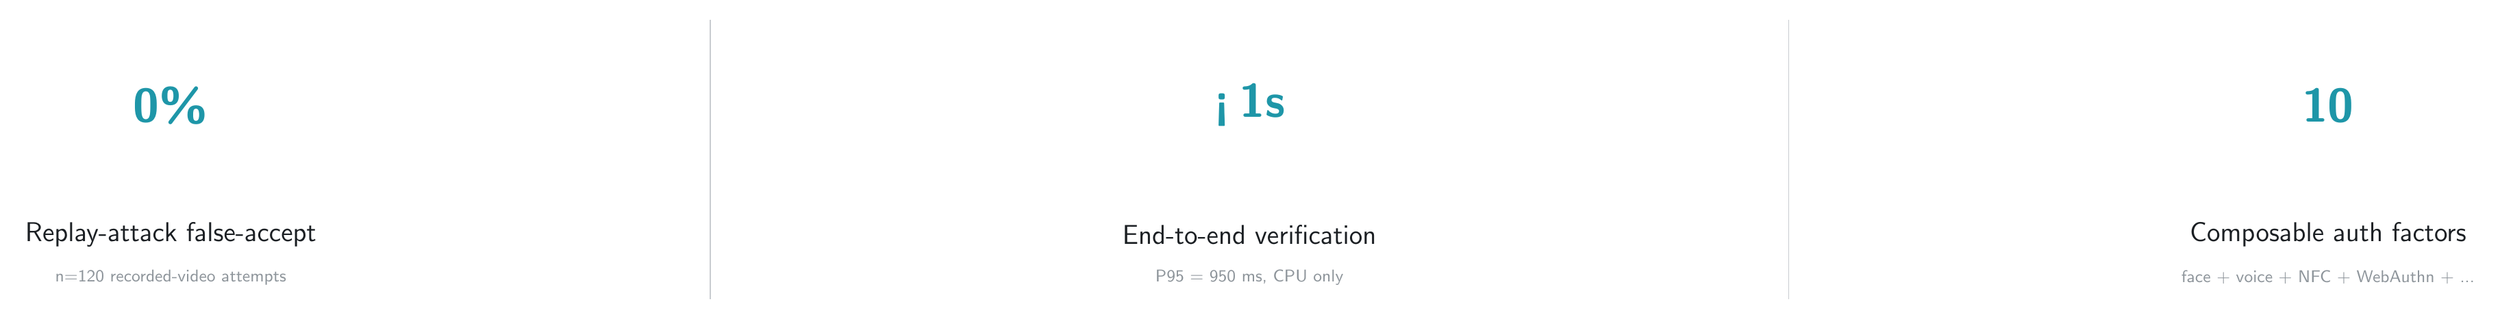
\begin{tikzpicture}[every node/.style={align=center}]
  \node[font=\fontsize{56}{56}\selectfont\bfseries, text=MAccent] (a) at (-20,0) {0\%};
  \node[font=\Large, text=MInk]            at (-20,-2.4) {Replay-attack false-accept};
  \node[font=\small, text=MGray]           at (-20,-3.2) {n=120 recorded-video attempts};

  \node[font=\fontsize{56}{56}\selectfont\bfseries, text=MAccent] (b) at ( 0,0) {<\,1s};
  \node[font=\Large, text=MInk]            at (  0,-2.4) {End-to-end verification};
  \node[font=\small, text=MGray]           at (  0,-3.2) {P95 = 950 ms, CPU only};

  \node[font=\fontsize{56}{56}\selectfont\bfseries, text=MAccent] (c) at (20,0) {10};
  \node[font=\Large, text=MInk]            at ( 20,-2.4) {Composable auth factors};
  \node[font=\small, text=MGray]           at ( 20,-3.2) {face + voice + NFC + WebAuthn + ...};

  \draw[draw=MRule, line width=0.6pt] (-10,-3.6) -- (-10,1.6);
  \draw[draw=MRule, line width=0.6pt] ( 10,-3.6) -- ( 10,1.6);
\end{tikzpicture}}

% ---------- Thin separator ---------------------------------------------------
\block[bodyoffsety=-2mm, bodyinnersep=0mm]{}{\centering

\begin{tikzpicture}\draw[MRule, line width=0.5pt] (0,0) -- (38,0);\end{tikzpicture}}

% ===================== COLUMNS ===============================================
\begin{columns}

% ---------------------- LEFT --------------------------------------------------
\column{0.5}

\block{}{\Large\bfseries\color{MAccent}01\quad\color{MInk}Problem\par\vspace{4mm}
\normalsize\color{MInk}\setlength{\parskip}{4pt}
Online authentication is fragmented. Passwords leak, SMS OTPs are SIM-swappable,
hardware keys exclude phone-only users, and most biometric services trust a
\textbf{single passive signal} — a still selfie or a recorded clip — that a
prepared attacker can replay.

GDPR and KVKK demand verifiable consent, right to erasure, and data
portability; consumer auth stacks treat these as an afterthought.

\vspace{3mm}\textbf{Goal.} A tenant-configurable, multi-modal identity
platform where any subset of ten authentication factors composes into MFA
flows — and where every biometric factor is protected by an \emph{active},
randomised liveness challenge a recorded video cannot replay.
\par\vspace{3mm}}

\block{}{\Large\bfseries\color{MAccent}02\quad\color{MInk}Architecture\par\vspace{6mm}
\centering
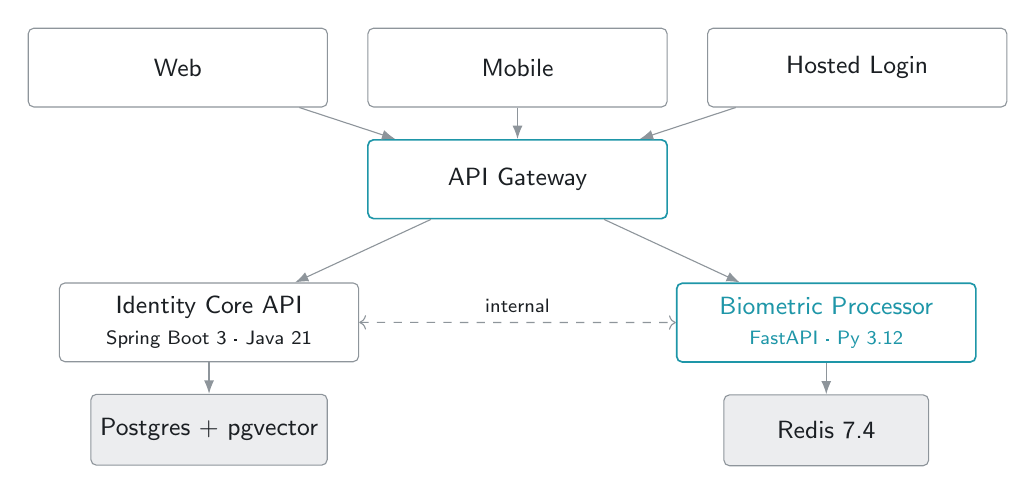
\begin{tikzpicture}[
  node distance=4mm and 5mm, every node/.style={font=\small, text=MInk},
  svc/.style ={draw=MGray, fill=MBg, rounded corners=2pt,
               minimum width=3.8cm, minimum height=1.0cm, align=center, line width=0.4pt},
  ml/.style  ={draw=MAccent, fill=MBg, rounded corners=2pt,
               minimum width=3.8cm, minimum height=1.0cm, align=center, line width=0.6pt, text=MAccent},
  data/.style={draw=MGray, fill=MGrayLite, rounded corners=2pt,
               minimum width=2.6cm, minimum height=0.9cm, align=center, line width=0.4pt},
  arrow/.style={-Latex, draw=MGray, line width=0.4pt},
]
\node[svc] (web)     {Web};
\node[svc, right=of web] (mobile) {Mobile};
\node[svc, right=of mobile] (widget) {Hosted Login};
\node[svc, below=of mobile, draw=MAccent, line width=0.6pt] (gw) {API Gateway};
\node[svc, below left=8mm and 0.1cm of gw] (api) {Identity Core API\\\scriptsize Spring Boot 3 · Java 21};
\node[ml,  below right=8mm and 0.1cm of gw] (bio) {Biometric Processor\\\scriptsize FastAPI · Py 3.12};
\node[data, below=of api]  (db)   {Postgres + pgvector};
\node[data, below=of bio]  (redis){Redis 7.4};
\foreach \src in {web,mobile,widget} {\draw[arrow] (\src) -- (gw);}
\draw[arrow] (gw) -- (api); \draw[arrow] (gw) -- (bio);
\draw[arrow] (api) -- (db); \draw[arrow] (bio) -- (redis);
\draw[arrow,<->,dashed] (api) -- node[above,sloped,font=\scriptsize]{internal} (bio);
\end{tikzpicture}\par\vspace{3mm}
\small\textcolor{MGray}{Biometric service has no public route — Docker network only, API-key gated.}
\par\vspace{3mm}}

\block{}{\Large\bfseries\color{MAccent}03\quad\color{MInk}Passive vs.\ active liveness\par\vspace{5mm}
\normalsize\color{MInk}
\begin{minipage}[t]{0.48\linewidth}
{\bfseries Passive only}\\[2mm]
\textcolor{MGray}{\small Single frame → texture / colour cues.}\\[3mm]
\faTimes\quad Photo of phone screen — \textit{often passes}\\[1mm]
\faTimes\quad Recorded clip — \textit{passes}\\[1mm]
\faTimes\quad Deepfake injection — \textit{often passes}
\end{minipage}\hfill\begin{minipage}[t]{0.48\linewidth}
{\bfseries\color{MAccent} Active challenge}\\[2mm]
\textcolor{MGray}{\small Randomised n-step facial-action sequence + landmarks + passive layer.}\\[3mm]
\faCheck\quad Photo — \textit{fails}\\[1mm]
\faCheck\quad Recorded clip — \textit{fails (sequence mismatch)}\\[1mm]
\faCheck\quad Deepfake — \textit{must hit cues live}
\end{minipage}
\par\vspace{3mm}}

% ---------------------- RIGHT -------------------------------------------------
\column{0.5}

\block{}{\Large\bfseries\color{MAccent}04\quad\color{MInk}Contributions\par\vspace{4mm}
\normalsize\color{MInk}
\begin{enumerate}[leftmargin=*, labelsep=8pt, label=\textcolor{MAccent}{\textbf{C\arabic*.}}, itemsep=4pt]
\item \textbf{Tenant-configurable composition} of 10 authentication factors into MFA flows declared at the admin layer.
\item \textbf{Active randomised liveness} — n-step facial-action sequence bound to a per-attempt nonce, verified server-side against landmark thresholds and temporal consistency.
\item \textbf{Pipeline decomposition} along the OIDC-contract / ML-iteration boundary into two horizontally-scalable services on a private Docker network.
\item \textbf{Embedding-at-rest encryption} — Facenet512 embeddings wrapped in Fernet (AES-128-CBC + HMAC-SHA-256) prior to write into pgvector.
\item \textbf{Regulator-aware data lifecycle} — tenant-scoped soft-delete, scheduled purge, audit-logging satisfying GDPR Art.\ 15 / 17 and KVKK.
\end{enumerate}
\par\vspace{3mm}}

\block{}{\Large\bfseries\color{MAccent}05\quad\color{MInk}Methods\par\vspace{4mm}
\normalsize\color{MInk}Per verification attempt:
\begin{enumerate}[leftmargin=*, labelsep=8pt, label=\textcolor{MAccent}{\bfseries\arabic*.}, itemsep=4pt]
\item Server issues a randomised action sequence (n=3–5) + nonce.
\item Client streams 60-frame landmark vectors (MediaPipe FaceLandmarker, 468 points).
\item Server checks each action against EAR / MAR / yaw thresholds + temporal consistency.
\item UniFace MiniFASNet runs a passive spoof check in parallel.
\item Embedding (Facenet512) encrypted with Fernet (AES-128-CBC + HMAC-SHA-256) and matched against the user vector in pgvector (HNSW).
\end{enumerate}
\par\vspace{4mm}\textcolor{MGray}{60 Flyway migrations · 5 submodules · self-hosted GitHub runner on Hetzner CX43 · 1\,820+ tests · 8 ADRs.}
\par\vspace{3mm}}

\block{}{\Large\bfseries\color{MAccent}06\quad\color{MInk}10 composable factors\par\vspace{5mm}
\centering\normalsize
\begin{tikzpicture}[every node/.style={font=\small, text=MInk, align=center},
  tile/.style={draw=MGray, line width=0.4pt, rounded corners=2pt,
               minimum width=4.6cm, minimum height=1.4cm, align=center},
  gtile/.style={draw=MAccent, line width=0.6pt, fill=MAccent!10, rounded corners=2pt,
                minimum width=4.6cm, minimum height=1.4cm, align=center, text=MInk}]
\node[tile] (n1) at (-9, 3)  {\faKey\ Password};
\node[tile] (n2) at ( 0, 3)  {\faEnvelope\ Email OTP};
\node[tile] (n3) at ( 9, 3)  {\faSms\ SMS OTP};
\node[tile] (n4) at (-9, 1)  {\faClock\ TOTP};
\node[tile] (n5) at ( 0, 1)  {\faQrcode\ QR};
\node[gtile] (n6) at ( 9, 1)  {\faSmile\ Face};
\node[gtile] (n7) at (-9,-1) {\faMicrophone\ Voice};
\node[gtile] (n8) at ( 0,-1) {\faFingerprint\ Fingerprint};
\node[tile] (n9) at ( 9,-1) {\faUsb\ WebAuthn};
\node[tile] (n10) at (0,-3) {\faIdCard\ NFC document (MRZ + chip)};
\end{tikzpicture}\par\vspace{3mm}
\small\textcolor{MGray}{Teal tiles = wrapped in active-liveness; any subset composes into a tenant MFA flow.}
\par\vspace{3mm}}

\block{}{\Large\bfseries\color{MAccent}07\quad\color{MInk}Experiments \& results\par\vspace{5mm}
\centering
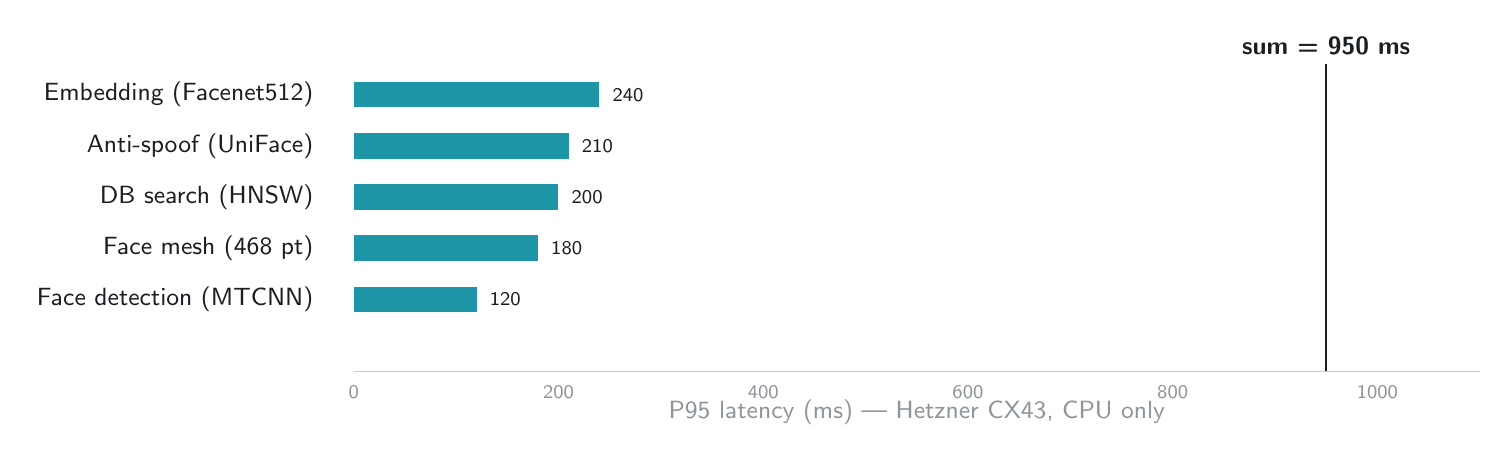
\begin{tikzpicture}[x=0.013cm, y=0.65cm,
  bar/.style={draw=none, fill=MAccent},
  axislabel/.style={font=\small, text=MInk, anchor=east},
  axislabelinside/.style={font=\scriptsize, anchor=west, text=MInk}]
\draw[MRule, line width=0.4pt] (0,-0.4) -- (1100,-0.4);
\foreach \x in {0,200,400,600,800,1000}{
  \node[font=\scriptsize, anchor=north, text=MGray] at (\x,-0.5) {\x};
}
\node[font=\small, text=MGray] at (550,-1.2) {P95 latency (ms) — Hetzner CX43, CPU only};
\node[axislabel] at (-30,5) {Embedding (Facenet512)};   \filldraw[bar] (0,4.75) rectangle (240,5.25); \node[axislabelinside] at (240,5.0) {\,240};
\node[axislabel] at (-30,4) {Anti-spoof (UniFace)};      \filldraw[bar] (0,3.75) rectangle (210,4.25); \node[axislabelinside] at (210,4.0) {\,210};
\node[axislabel] at (-30,3) {DB search (HNSW)};          \filldraw[bar] (0,2.75) rectangle (200,3.25); \node[axislabelinside] at (200,3.0) {\,200};
\node[axislabel] at (-30,2) {Face mesh (468 pt)};        \filldraw[bar] (0,1.75) rectangle (180,2.25); \node[axislabelinside] at (180,2.0) {\,180};
\node[axislabel] at (-30,1) {Face detection (MTCNN)};    \filldraw[bar] (0,0.75) rectangle (120,1.25); \node[axislabelinside] at (120,1.0) {\,120};
\draw[MInk, line width=0.6pt] (950,-0.4) -- (950,5.6);
\node[font=\small\bfseries, text=MInk, anchor=south] at (950,5.6) {sum = 950 ms};
\end{tikzpicture}
\par\vspace{4mm}\setlength{\tabcolsep}{6pt}\renewcommand{\arraystretch}{1.2}\normalsize
\begin{tabular}{@{}l r r@{}}
\textcolor{MGray}{Quality metric}            & \textcolor{MGray}{Target} & \textcolor{MGray}{Observed} \\[1pt]
Replay-attack FAR (n=120)                    & {<}\,1\%         & \textbf{0.0\%} \\
Passive-spoof AUC (internal)                 & {>}\,0.95        & \textbf{0.97} \\
Backend tests                                & green            & 633 / 633 \\
Web Vitest + Playwright                      & green            & 619 + 27 \\
Mobile (KMP) units                           & green            & 425 / 425 \\
\end{tabular}
\par\vspace{3mm}}

\block{}{\Large\bfseries\color{MAccent}08\quad\color{MInk}Conclusion\par\vspace{4mm}
\normalsize\color{MInk}
Production-grade, GDPR-compliant biometric authentication \emph{is} achievable on commodity
hardware when the system is decomposed along its right axis — a frozen OIDC contract on one
side, an iterating ML pipeline on the other — and when liveness is treated as an active,
challenge-driven property rather than a passive signal alone. Measured 0\,/\,120 replay-attack
false-accepts and a 0.97 passive-spoof AUC are both within practical deployment limits on a
single CPU server.
\par\vspace{3mm}}

\block{}{\Large\bfseries\color{MAccent}09\quad\color{MInk}Future work\par\vspace{4mm}
\normalsize\color{MInk}
\begin{itemize}[leftmargin=*, labelsep=8pt, label=\textcolor{MAccent}{\textbf{—}}, itemsep=3pt]
\item \textbf{BYOD tenant DB.} Enterprise tenants host biometric data in their own database, schema-pinned.
\item \textbf{On-device pre-filter.} Stripped MediaPipe pipeline drops obvious non-faces before upload — bandwidth + privacy win.
\item \textbf{Cross-modal challenge.} Voice nonce + facial action to defeat audio-only deepfakes.
\item \textbf{Verifiable credentials.} W3C VCs after successful KYC for downstream-service portability.
\end{itemize}}

\end{columns}

% ---------- Bottom row: QR + refs --------------------------------------------
\block[bodyoffsety=-2mm, bodyinnersep=0mm]{}{\centering

\begin{tikzpicture}\draw[MRule, line width=0.5pt] (0,0) -- (38,0);\end{tikzpicture}}

\block[bodyoffsety=4mm, bodyinnersep=6mm]{}{%
\begin{minipage}[t]{0.22\linewidth}\centering
\qrcode[height=4.2cm,version=4,level=H]{https://verify.fivucsas.com}\\[2mm]
{\small\color{MGray}\faCamera\ Scan for live demo}\\
{\small\bfseries\color{MInk}verify.fivucsas.com}
\end{minipage}\hfill\begin{minipage}[t]{0.74\linewidth}\small\color{MInk}
{\bfseries\color{MAccent}References}\\[2mm]
\begin{enumerate}[leftmargin=*, labelsep=6pt, label=\textcolor{MGray}{[\arabic*]}, itemsep=1pt]
\item Serengil, S., Özpınar, A. \textit{LightFace / DeepFace}. IEEE ASYU, 2020.
\item Lugaresi, C.\ et al. \textit{MediaPipe: A Framework for Building Perception Pipelines.} arXiv:1906.08172.
\item Soukupová, T., Čech, J. \textit{Real-Time Eye Blink Detection using Facial Landmarks.} CVWW, 2016.
\item Wan, L.\ et al. \textit{Generalized End-to-End Loss for Speaker Verification.} ICASSP, 2018.
\item Yadav, S.\ et al. \textit{UniFace: A Unified Architecture for Face Spoofing Detection.} CVPR-W, 2023.
\end{enumerate}
\end{minipage}
\par\vspace{8mm}\centering\small\color{MGray}
\faGithub\ github.com/Rollingcat-Software/FIVUCSAS \quad·\quad
\faGlobe\ fivucsas.com \quad·\quad
\faEnvelope\ ahmetabdullahgultekin@gmail.com \quad·\quad
Marmara University \textbf{2026}
}

\end{document}
